\documentclass[11pt,a4paper]{article}
\usepackage[a4paper,margin=1in]{geometry}
\usepackage{times}
\usepackage[round]{natbib}
\usepackage{setspace}
\onehalfspacing

\usepackage{hyperref}
\usepackage{url}
\usepackage{graphicx}
\usepackage{booktabs}
\usepackage{subcaption}
\usepackage{amsmath}
\usepackage{amssymb}
\usepackage{amsthm}
\usepackage{algorithm}
\usepackage{algpseudocode}
\usepackage{tikz}
\usetikzlibrary{arrows.meta,positioning,fit,backgrounds,calc}
\urlstyle{rm}

\newtheorem{definition}{Definition}
\newtheorem{proposition}{Proposition}
\newtheorem{remark}{Remark}

\newcommand{\CutWorld}{\textsc{CutWorld}}
\newcommand{\BnC}{B\&C}
\newcommand{\argmax}{\operatorname*{arg\,max}}
\newcommand{\softmax}{\operatorname{softmax}}
\newcommand{\SGM}{\operatorname{SGM}}
\newcommand{\fracset}{\mathcal{F}}
\newcommand{\R}{\mathbb{R}}

% -----------------------------------------------------------------------
\title{\textbf{CutWorld: A Latent Dynamics Model for Unified Branch-and-Cut Control}\\[1.5em]
\large M.Tech Project Report}

% Fill in your details below.
\author{[Student Name] \\ [Roll Number] \\[1em]
Supervisor: [Supervisor Name] \\[1em]
[Department] \\ [Institute]}

\date{\today}
% -----------------------------------------------------------------------

\begin{document}

\maketitle
\thispagestyle{empty}

\begin{abstract}
Branch-and-Cut solvers repeatedly choose a branching variable, a cutting plane, and an open search node. These choices reshape an exponentially large search tree, but standard learned branching rules score candidates only from the current relaxation. We present \CutWorld{}, a latent decision-dynamics model that plans over candidate branching actions without solving their child linear programs. A bipartite GATv2 encoder maps the current relaxation to a global latent and per-variable embeddings. A causal Transformer then predicts the latent successor and its variable embeddings conditioned on a candidate and branch direction, allowing the policy to be re-applied to imagined states. We combine the resulting rollout value with the predicted dual-bound progress and cost-to-go, and use the shared representation to order nodes and select the root Gomory cut. Because the learned components only select among valid branches, globally valid cuts, and open-node orderings, they do not alter feasibility or bound tests. We evaluate on 30 medium ($500\times1000$, 300\,s limit) and 15 hard ($1000\times2000$, 600\,s limit) Set Cover instances drawn from three generator seeds, against most-fractional and strong-branching rules in the same Python/HiGHS harness and against SCIP. No method, SCIP included, closes these instances within the budget, so we compare primal and proven gaps at equal time using paired statistical tests. Combining the learned policy with most-fractional ranking significantly improves on the imitation policy on both tiers (proven gap 19.1\% versus 23.3\% at medium scale and 31.7\% versus 35.5\% at hard scale) and comes within 0.1 percentage points of most-fractional branching at hard scale, while most-fractional remains the strongest rule in the harness. Model inference accounts for most of the per-node cost, and an ablation shows that the cut-selection rule has no significant effect on this cut pool. We report the full evaluation pipeline, including an independent feasibility check of every returned solution, and discuss what the results imply for latent planning in exact tree search.
\end{abstract}

\newpage
\tableofcontents
\newpage

% -----------------------------------------------------------------------
\section{Introduction}

A modern optimization solver makes millions of discrete sequential choices to solve a single instance, like which variable
to branch on, which cutting planes to add, which open node to explore next,
each one steering an enormous combinatorial search, and each governed today by a
hand-engineered heuristic. Model-based planning agents such as MuZero and
Dreamer \citep{schrittwieser2020mastering,hafner2020dream} have shown that
learning a model of environment dynamics, and planning by imagining the
consequences of actions, transforms sequential decision making, from Atari and
Go to continuous control. We bring this idea inside an optimization solver:
\emph{CutWorld}, a latent dynamics model for unified Branch-and-Cut control.

Mixed-Integer Programming (MIP) is a cornerstone of combinatorial optimization,
and modern solvers attack it with Branch-and-Cut. Starting from a linear
programming (LP) relaxation, B\&C repeatedly executes two core operations at
each search tree node: adding cutting planes, valid inequalities that tighten
the relaxation without removing integer solutions, and branching on a fractional
variable to partition the search space.

Unfortunately, making high-quality decisions at every node is computationally
expensive. The gold standard for branching, \emph{strong branching}, tentatively
solves the child LPs of each candidate variable to measure its bound
improvement; cut selection faces an analogous trade-off when choosing among
large pools of valid inequalities. To amortize these costs, recent machine
learning approaches learn to imitate strong branching in a single forward pass,
e.g., with graph neural networks \citep{gasse2019exact,khalil2016learning}, or
use reinforcement learning to select cuts \citep{tang2020reinforcement}. These
methods are effective, but they share a structural limitation: each scores a
candidate \emph{from the current node alone}, discarding the lookahead
signal.

CutWorld closes this gap with a learned latent dynamics model. We encode each
search node as a bipartite graph with a GATv2 network and attention readout,
and train a causal Transformer to predict how the latent and per-variable
embeddings evolve under a candidate action, so the branching policy can be
re-applied to imagined states for a k-step rollout. Candidates are scored by a
MuZero-style return combining predicted rewards, a value estimate, and a
cost-to-go penalty; Gomory cuts are selected via cross-attention over the same
encoder representations. A single unified model drives variable branching, cut
selection, and node ordering while preserving the solver's exactness guarantee.

\paragraph{Contributions.}
\begin{itemize}
  \item We formulate learned \BnC{} control as latent decision dynamics and introduce a per-variable transition model that supports policy reapplication in imagined states.
  \item We derive a search-aware rollout objective that combines predicted dual-bound progress, value bootstrap, and cost-to-go, and provide a correctness argument for using learned decisions within exact tree search.
  \item We implement shared latent control of branching, node ordering, and root Gomory-cut selection in a single Python/HiGHS research harness.
  \item We provide a controlled Set Cover study on 45 instances from three generator seeds, with classical and SCIP baselines, equal-time gap comparisons, paired statistical tests, an ablation of the cut-selection rule, and per-node measurements of solver and model time.
\end{itemize}

% -----------------------------------------------------------------------
\section{Related Work}

\paragraph{Learning to branch.}
Early work learned branching scores from hand-crafted MIP features \citep{khalil2016learning}. Gasse et al.~\citep{gasse2019exact} introduced a bipartite graph representation of variables and constraints and trained a graph convolutional policy to imitate strong branching. This representation is the starting point for our encoder, while our central difference is a learned transition model that is used after training for prospective lookahead. Tree-structured returns \citep{scavuzzo2022learning} and neural diving and branching \citep{nair2020solving} demonstrate the value of longer-horizon objectives, but do not model the solver transition explicitly. The broader methodological landscape is surveyed by \citet{bengio2021machine}.

\paragraph{Learning to cut and optimize.}
Cut selection has been formulated as reinforcement learning
\citep{tang2020reinforcement}, imitation from cut lookahead
\citep{paulus2022learning}, and hierarchical sequence prediction \citep{wang2023hierarchical}. These approaches motivate our use of candidate-level cut features, but our deployment restricts the learner to selecting from a pool of validity-certified Gomory cuts. Learned large neighborhood search provides another example of learned solver control \citep{sonnerat2021learning}. We focus instead on exact tree search, where learned decisions must remain separate from pruning and feasibility logic.

\paragraph{Sequence models and model-based planning.}
Mamba-Branching models realized branching histories with a state-space model \citep{zhang2026mambabranchin}. Such retrospective history modeling complements our prospective model: we predict the consequences of an unrealized action before committing to it. \CutWorld{} follows the latent planning principle of MuZero and Dreamer
\citep{schrittwieser2020mastering,hafner2020dream}, but the state is a constraint--variable relaxation and the action space is solver-specific.


\section{Background and Problem Formulation}
\label{sec:background}

\subsection{Mixed-Integer Programming and Branch-and-Cut}

We study binary MIPs of the form
\begin{equation}
  \min_{x\in\{0,1\}^{n}} c^\top x
  \quad\text{s.t.}\quad
  Ax\ge b,
  \qquad
  A\in\R^{m\times n},\ c\in\R^n,\ b\in\R^m .
  \label{eq:mip}
\end{equation}
Set Cover is the special case $A\in\{0,1\}^{m\times n}$ and
$b=\mathbf{1}$. At a search node $u$, the integer restrictions are relaxed
and the solver obtains
\begin{equation}
  \ell(u)=\min_{x\in[0,1]^n} c^\top x
  \quad\text{s.t.}\quad A_u x\ge b_u .
  \label{eq:lp}
\end{equation}
If $x_u^\star$ is fractional, branching on $j$ creates two descendants with $x_j\le 0$ and $x_j\ge 1$ (equivalently, $x_j=0$ and $x_j=1$ for binary variables). A valid cut $\alpha^\top x\ge\beta$ tightens the LP relaxation without removing any integer-feasible point.

For a node with incumbent objective $U$ and dual bound $\ell(u)$, the relative primal--dual gap is
\begin{equation}
  g(u)=\frac{|U-\ell(u)|}{\max\{1,|U|\}} .
  \label{eq:gap}
\end{equation}
The learned policy never computes $g(u)$ and never changes the bound, integrality, or feasibility tests. It only selects actions and open-node orderings.

\subsection{A Latent Decision Process}

We represent a search state $s_t$ by the current relaxation graph, its LP
solution, and its root-to-node decision history. The action is
$a_t=(v_t,d_t)$, where $v_t$ is a fractional variable and
$d_t\in\{-1,+1\}$ is the branch direction. Cuts are treated as a
validity-certified auxiliary action at the root. The solver induces a
transition $P(s_{t+1}\mid s_t,a_t)$ by solving the child relaxation.

The objective is to reduce search effort while preserving correctness. We use
dual-bound progress as a dense auxiliary reward,
\begin{equation}
  r_t=\operatorname{norm}\!\left(\ell(s_{t+1})-\ell(s_t)\right),
  \qquad
  J=\mathbb{E}\!\left[\sum_{t=0}^{T-1}\gamma^t r_t
      -\eta\,\log(1+N_{\mathrm{tree}})\right],
  \label{eq:mdp-return}
\end{equation}
where $N_{\mathrm{tree}}$ is the number of search-tree nodes processed and
$\eta$ controls the search-cost auxiliary. The true transition is expensive;
\CutWorld{} learns a latent approximation $\widehat P$.

\begin{proposition}[Correctness under admissible control]
\label{prop:correctness}
Assume that (i) every branching variable is selected from the current fractional binary variables, (ii) every added cut is globally valid for the original integer-feasible set, and (iii) pruning is performed only from certified infeasibility, integrality, or valid bound comparisons. Then, replacing the baseline branching rule, cut ordering, or open-node ordering by any \CutWorld{} policy preserves the set of optimal integer solutions returned by Branch-and-Cut.
\end{proposition}




\section{CutWorld}
\label{sec:method}

\begin{figure*}[t]
\centering
\resizebox{\linewidth}{!}{
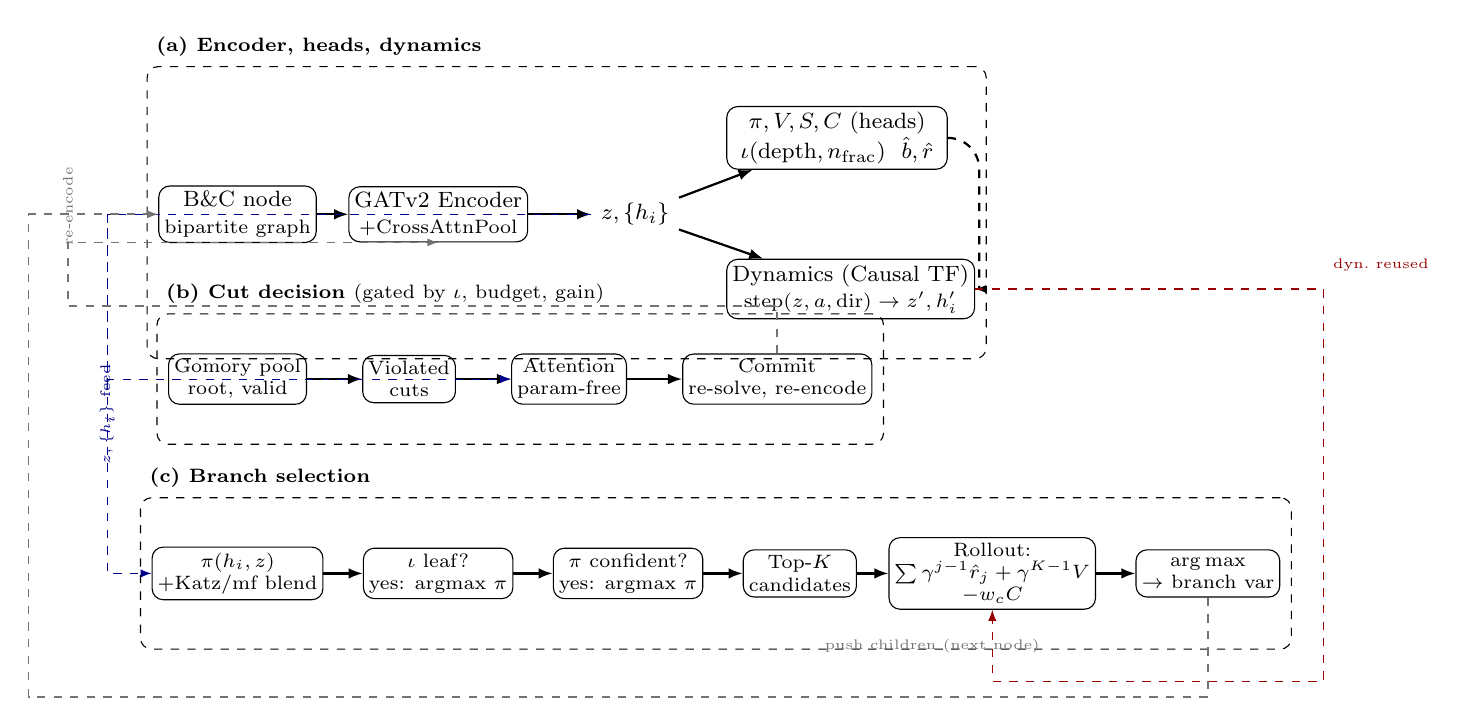
\begin{tikzpicture}[
  node distance=3mm and 4mm,
  box/.style={draw, rounded corners, align=center, minimum height=7mm,
              inner sep=2pt, font=\footnotesize},
  small/.style={draw, rounded corners, align=center, minimum height=6mm,
              inner sep=2pt, font=\scriptsize},
  lat/.style={align=center, font=\footnotesize},
  panel/.style={draw, dashed, rounded corners, inner xsep=4pt, inner ysep=5mm},
  ptitle/.style={font=\scriptsize\bfseries, anchor=south west},
  arr/.style={-{Latex[length=1.8mm]}, thick},
  thinarr/.style={-{Latex[length=1.4mm]}},
  feed/.style={thinarr, dashed, blue!55!black},
  reuse/.style={thinarr, dashed, red!60!black},
  loop/.style={thinarr, dashed, black!55, line width=0.6pt},
]

% ---------- Panel (a): core architecture ----------
\node[box] (inp) {B\&C node\\{\scriptsize bipartite graph}};
\node[box, right=of inp] (enc) {GATv2 Encoder\\{\scriptsize +CrossAttnPool}};
\node[lat, right=8mm of enc] (z) {$z,\{h_i\}$};
\node[box, above right=3mm and 6mm of z, minimum width=28mm] (heads)
  {$\pi,V,S,C$ (heads)\\$\iota(\text{depth},n_{\text{frac}})$\ \ $\hat b,\hat r$};
\node[box, below right=3mm and 6mm of z, minimum width=28mm] (dyn)
  {Dynamics (Causal TF)\\{\scriptsize step$(z,a,\text{dir})\to z',h_i'$}};

\draw[arr] (inp) -- (enc);
\draw[arr] (enc) -- (z);
\draw[arr] (z) -- (heads);
\draw[arr] (z) -- (dyn);
\draw[arr, thinarr, dashed] (heads.east) to[out=0,in=90] ++(4mm,-4mm) |- (dyn.east);

\node[panel, fit=(inp)(enc)(z)(heads)(dyn)] (panelA) {};
\node[ptitle] at (panelA.north west) {(a) Encoder, heads, dynamics};

% ---------- Panel (b): cut decision ----------
\node[small, below=14mm of inp] (pool) {Gomory pool\\{\scriptsize root, valid}};
\node[small, right=7mm of pool] (viol) {Violated\\cuts};
\node[small, right=7mm of viol] (attn) {Attention\\{\scriptsize param-free}};
\node[small, right=7mm of attn] (commit) {Commit\\{\scriptsize re-solve, re-encode}};

\draw[arr] (pool) -- (viol);
\draw[arr] (viol) -- (attn);
\draw[arr] (attn) -- (commit);

\node[panel, fit=(pool)(viol)(attn)(commit)] (panelB) {};
\node[ptitle] at (panelB.north west) {(b) Cut decision\ {\normalfont\scriptsize(gated by $\iota$, budget, gain)}};

% ---------- Panel (c): branch selection ----------
\node[small, below=18mm of pool] (pscore) {$\pi(h_i,z)$\\{\scriptsize +Katz/mf blend}};
\node[small, right=5mm of pscore] (leafchk) {$\iota$ leaf?\\{\scriptsize yes: argmax $\pi$}};
\node[small, right=5mm of leafchk] (confchk) {$\pi$ confident?\\{\scriptsize yes: argmax $\pi$}};
\node[small, right=5mm of confchk] (topk) {Top-$K$\\candidates};
\node[small, right=4mm of topk, minimum width=26mm] (roll)
  {Rollout:\\$\sum\gamma^{j-1}\hat r_j + \gamma^{K-1}V$\\$- w_cC$};
\node[small, right=5mm of roll] (argmax) {$\arg\max$\\$\to$ branch var};

\draw[arr] (pscore) -- (leafchk);
\draw[arr] (leafchk) -- (confchk);
\draw[arr] (confchk) -- (topk);
\draw[arr] (topk) -- (roll);
\draw[arr] (roll) -- (argmax);

\node[panel, fit=(pscore)(leafchk)(confchk)(topk)(roll)(argmax)] (panelC) {};
\node[ptitle] at (panelC.north west) {(c) Branch selection};

% ---------- Cross-panel interconnections ----------
\coordinate (rbus) at ($(panelC.east)+(4mm,0)$);
\draw[reuse] (dyn.east) -| (rbus |- panelC.south) -- ++(0,-4mm) -| (roll.south);
\node[font=\tiny, red!60!black, anchor=west] at ($(dyn.east -| rbus)+(0,3mm)$) {dyn.\ reused};

\coordinate (lbus) at ($(panelA.west)+(-5mm,0)$);
\draw[feed] (z.west) -- (z.west -| lbus)
            -- (attn.west -| lbus) -- (attn.west);
\draw[feed] (z.west -| lbus) -- (pscore.west -| lbus) -- (pscore.west);
\node[font=\tiny, blue!55!black, anchor=east, rotate=90] at ($(lbus)+(0,-18mm)$) {$z,\{h_i\}$ feed};

\coordinate (lbus2) at ($(panelA.west)+(-10mm,0)$);
\coordinate (commitN) at ($(commit.north)+(0,6mm)$);
\draw[loop] (commit.north) -- (commitN) -- (commitN -| lbus2)
            -- (enc.south -| lbus2) -- (enc.south);
\node[font=\tiny, black!55, anchor=east, rotate=90] at ($(lbus2)+(0,7mm)$) {re-encode};

\coordinate (fbus) at ($(panelA.west)+(-15mm,0)$);
\coordinate (bbus) at ($(panelC.south)+(0,-6mm)$);
\draw[loop] (argmax.south) -- (argmax.south |- bbus)
            -- (fbus |- bbus) -- (fbus |- inp.west) -- (inp.west);
\node[font=\tiny, black!55, anchor=north] at ($(argmax.south)+(-35mm,-4mm)$) {push children (next node)};

\end{tikzpicture}
}
\caption{\textbf{CutWorld architecture and decision pipeline.}
\textbf{(a)} A GATv2 encoder produces graph latent $z$ and per-variable embeddings $\{h_i\}$; a causal Transformer predicts their evolution under candidate actions.
\textbf{(b)} Valid Gomory cuts are selected by attention, subject to integrality, budget, gain, and depth checks, then committed with an LP re-solve.
\textbf{(c)} Fractional variables are scored by $\pi$; confident nodes exit early, while ambiguous nodes use latent rollout with repeated policy re-application and reward/cost-to-go scoring.
Dashed links indicate shared representations ($z,\{h_i\}$) and dynamics reuse; gray loops denote cut re-solving and branch-node expansion. Learned components only select valid actions and do not alter LP bounds or feasibility tests.}
\label{fig:arch}
\end{figure*}

We view Branch-and-Cut as a sequential decision process. At each node $t$ of the search, the solver observes a state $s_t$ (the current relaxation), takes an action $a_t$ (branch on a fractional variable, or add a cut), and transitions to the next node. We learn (i)~an encoder that maps $s_t$ to a latent state, (ii)~a dynamics model that predicts how that latent evolves under an action, and (iii)~heads that score decisions by rolling the dynamics forward (Figure~\ref{fig:arch}). Throughout, $d=128$ denotes the embedding dimension.

\subsection{Bipartite Node Encoder}

The relaxation is a bipartite graph
$G_t=(\mathcal{V}_t,\mathcal{C}_t,\mathcal{E}_t)$ over variables and constraints. Each variable node contains objective, bound, LP solution, fractionality, reduced cost, and basis features; each constraint node contains normalized right-hand side, tightness, dual, and age features. Each edge contains its coefficient, a right-hand-side-normalized coefficient, and its sign. We use $19$ variable features, $5$ constraint features, and a three-dimensional edge feature.

Let $h_v^{(0)}$ and $h_i^{(0)}$ denote initial variable and constraint embeddings. A GATv2 layer computes attention coefficients
\begin{equation}
  \alpha_{iv}^{(\ell)}
  =
  \frac{\exp\left(
    a^\top \operatorname{LeakyReLU}
    \left(W_c h_i^{(\ell)}+W_v h_v^{(\ell)}
          +W_e e_{iv}\right)\right)}
  {\sum_{k\in\mathcal{N}(v)}
    \exp\left(
    a^\top \operatorname{LeakyReLU}
    \left(W_c h_k^{(\ell)}+W_v h_v^{(\ell)}
          +W_e e_{kv}\right)\right)}
  \label{eq:attention}
\end{equation}
and updates the two node types by normalized aggregation:
\begin{align}
  \widetilde h_v^{(\ell+1)}
    &=\sum_{i\in\mathcal{N}(v)}
       \alpha_{iv}^{(\ell)}W_c h_i^{(\ell)}, &
  h_v^{(\ell+1)}
    &=\operatorname{LN}\!\left(
      h_v^{(\ell)}+\operatorname{MLP}_v(\widetilde h_v^{(\ell+1)})
      \right), \\
  \widetilde h_i^{(\ell+1)}
    &=\sum_{v\in\mathcal{N}(i)}
       \alpha_{vi}^{(\ell)}W_v h_v^{(\ell)}, &
  h_i^{(\ell+1)}
    &=\operatorname{LN}\!\left(
      h_i^{(\ell)}+\operatorname{MLP}_c(\widetilde h_i^{(\ell+1)})
      \right).
  \label{eq:gnn-update}
\end{align}
The implementation uses three layers and four attention heads with $d=128$. A learned query $q$ pools the variable embeddings:
\begin{align}
  \omega_i&=
  \softmax_i\!\left(\frac{(W_q q)^\top(W_k h_i)}{\sqrt d}\right), &
  z_t&=\sum_{i=1}^{n}\omega_i W_v h_i, &
  \operatorname{Enc}(s_t)&=(z_t,\{h_i\}_{i=1}^{n}).
  \label{eq:pool}
\end{align}
Unlike a uniform mean, Eq.~\eqref{eq:pool} can emphasize variables that are fractional, expensive, or structurally connected to tight constraints.

\subsection{Latent Dynamics}

The action embedding concatenates the selected variable representation and a direction code:
\begin{equation}
  a_t=W_a\,[h_{v_t}\,\|\,\operatorname{onehot}(d_t)].
  \label{eq:action}
\end{equation}
The causal Transformer receives tokens
\begin{equation}
  u_\tau=W_{\mathrm{in}}
  [z_\tau\,\|\,a_\tau\,\|\,\operatorname{onehot}(d_\tau)]
  +p_\tau ,
  \qquad \tau\le t ,
  \label{eq:token}
\end{equation}
where $p_\tau$ is a learned positional embedding. A four-layer, four-head Transformer predicts a residual successor:
\begin{align}
  \Delta z_{t+1}
    &=W_z\,\operatorname{TF}_{\mathrm{causal}}(u_{0:t}), &
  \widehat z_{t+1}
    &=\operatorname{LN}(z_t+\Delta z_{t+1}).
  \label{eq:latent-transition}
\end{align}
The per-variable transition is
\begin{equation}
  \widehat h_i^{\,t+1}
  =
  \operatorname{LN}\!\left(
    h_i^t+
    \operatorname{MLP}_h
      [h_i^t\,\|\,\widehat z_{t+1}\,\|\,a_t]
  \right).
  \label{eq:variable-transition}
\end{equation}
This factorization is important: a graph-level prediction alone cannot re-score the candidate variables at the imagined state.

Two grounding heads connect the latent to solver quantities:
\begin{equation}
  \widehat \ell_{t+1}=w_\ell^\top\widehat z_{t+1},
  \qquad
  \widehat r_t=w_r^\top\widehat z_{t+1}.
  \label{eq:grounding}
\end{equation}

\subsection{Policy, Value, and Cost-to-Go Heads}

Let $\bar h_{\mathrm{frac}}$ be the mean embedding of currently fractional variables. The value and cost-to-go heads use this state-dependent summary:
\begin{align}
  V(s_t)&=f_V([z_t\,\|\,\bar h_{\mathrm{frac}}]), &
  C(s_t)&=\operatorname{softplus}
       \left(f_C([z_t\,\|\,\bar h_{\mathrm{frac}}])\right).
  \label{eq:value-cost}
\end{align}
The target for $C$ is $\log(1+T-t)$, where $T-t$ is the number of remaining transitions in a trajectory. The policy is a pointer scorer over $i\in\fracset_t$:
\begin{align}
  k_i&=W_kh_i, &
  \ell_i&=
  \frac{w_\pi^\top
    \tanh(k_i+W_zz_t)}{\sqrt d}, &
  \pi(i\mid s_t)&=\softmax_{i\in\fracset_t}(\ell_i).
  \label{eq:policy}
\end{align}
An integrality head predicts whether the current node is close to terminal:
\begin{equation}
  p_{\mathrm{leaf}}(s_t)=
  \sigma\!\left(
    f_{\mathrm{int}}
      [z_t\,\|\,\operatorname{depth}(t)/D\,\|\,\log(1+n_{\mathrm{frac}})]
  \right).
  \label{eq:integrality}
\end{equation}
It is used only as a computational gate; it cannot certify a node or trigger
unsafe pruning.

\subsection{Latent Rollout and Node Ordering}

For a candidate $c$, the model takes $a_0=h_c$ and recursively predicts $K$ imagined states. At each imagined state, the policy chooses the next action from the predicted fractional set. A depth-$K$ score is
\begin{equation}
  R_K(c)=
  \sum_{j=1}^{K}\gamma^{j-1}\widehat r_j
  +\gamma^{K}V(\widehat s_K)
  -w_C\sum_{j=1}^{K}\gamma^{j-1}\widehat C(\widehat s_j).
  \label{eq:rollout}
\end{equation}
The terminal value is discounted once for each latent transition. For a candidate set $\mathcal{C}_t=\operatorname{TopK}_k(\pi,\fracset_t)$, we standardize policy logits and rollout scores within the candidate set and select
\begin{equation}
  c^\star=
  \argmax_{c\in\mathcal{C}_t}
    \left[
      \operatorname{zscore}(\ell_c)
      +\lambda\operatorname{zscore}(R_K(c))
    \right].
  \label{eq:anchored-policy}
\end{equation}
When the policy is sufficiently confident, the rollout is skipped. Open nodes are ordered by predicted cost-to-go, with certified lower bounds retained as a secondary key.

\begin{algorithm}[t]
\caption{Policy-anchored latent branching}
\label{alg:branch}
\begin{algorithmic}[1]
\Require Encoded state $(z,\{h_i\})$, fractional set $\fracset$, horizon $K$,
         candidate budget $k$, rollout weight $\lambda$
\State $\ell_i\gets$ policy logits from Eq.~\eqref{eq:policy}
\If{$\max_{i\in\fracset}\softmax(\ell)_i\ge\theta$}
  \State \Return $\argmax_{i\in\fracset}\ell_i$
\EndIf
\State $\mathcal{C}\gets\operatorname{TopK}_k(\ell,\fracset)$
\For{$c\in\mathcal{C}$}
  \State $\widehat R(c)\gets$ latent rollout from Eq.~\eqref{eq:rollout}
\EndFor
\State Normalize $\ell_c$ and $\widehat R(c)$ over $\mathcal{C}$
\State \Return $\argmax_{c\in\mathcal{C}}
  [\operatorname{zscore}(\ell_c)+\lambda\operatorname{zscore}(\widehat R(c))]$
\end{algorithmic}
\end{algorithm}

\subsection{Root Gomory-Cut Selection}

\CutWorld{} selects cuts from a validity-certified root pool. Let a basic tableau row of the root LP be
\begin{equation}
  x_B+\sum_{j\in\mathcal{N}} \bar a_j x_j=\bar b,
  \qquad x_B\notin\mathbb{Z},\quad \bar b\notin\mathbb{Z}.
  \label{eq:tableau}
\end{equation}
Writing $\operatorname{frac}(q)=q-\lfloor q\rfloor$, the Gomory fractional
cut is
\begin{equation}
  \sum_{j\in\mathcal{N}}
      \operatorname{frac}(\bar a_j)x_j
  \ge
      \operatorname{frac}(\bar b).
  \label{eq:gomory}
\end{equation}
We express the cut in the original structural variables and retain it only when the generator's validity checks pass. A cut feature vector contains violation, efficacy, density, objective cutoff, support fraction, and parallelism. A parameter-free attention score is
\begin{equation}
  q_\ell=\frac{(W_c\phi_\ell)^\top(W_z z_t)}{\sqrt d},
  \qquad
  \rho_\ell=\softmax_\ell(q_\ell),
  \label{eq:cut-score}
\end{equation}
and the highest-scoring cut is committed, subject to the cut budget. This is a root cut selection, not a claim that a new separator is learned at every descendant. The distinction matters for both validity and computational cost.

\subsection{Training Objectives}
\label{sec:objectives}

The policy imitates strong branching with a hard-label cross-entropy and a soft target derived from normalized expert scores:
\begin{equation}
  \mathcal{L}_{\pi}
  =
  \operatorname{CE}(\pi,y_{\mathrm{SB}})
  +\alpha\,
    \operatorname{KL}\!\left(
      \softmax(\widetilde q_{\mathrm{SB}})
      \,\middle\|\,\pi
    \right).
  \label{eq:policy-loss}
\end{equation}
The value and cost-to-go losses use the Huber penalty
\begin{equation}
  \mathcal{H}_\delta(e)=
  \begin{cases}
    \frac12 e^2,& |e|\le\delta,\\
    \delta\left(|e|-\frac12\delta\right),& |e|>\delta,
  \end{cases}
  \quad
  \mathcal{L}_V=\mathcal{H}_\delta(V-\bar\ell),
  \quad
  \mathcal{L}_C=\mathcal{H}_\delta(C-\log(1+T-t)).
  \label{eq:huber}
\end{equation}
The one-step dynamics objective combines latent, variable, grounding, and reward terms:
\begin{align}
  \mathcal{L}_{\mathrm{dyn}}
  &=
  \|\widehat z_{t+1}-z_{t+1}\|_2^2
  +\beta_h\frac1n\sum_i
    \|\widehat h_i^{\,t+1}-h_i^{t+1}\|_2^2 \nonumber\\
  &\quad
  +\beta_\ell\mathcal{H}_\delta(\widehat\ell_{t+1}-\ell_{t+1})
  +\beta_r\mathcal{H}_\delta(\widehat r_t-r_t)
  +\beta_{\cos}
    \left(1-\cos(\widehat z_{t+1},z_{t+1})\right).
  \label{eq:dynamics-loss}
\end{align}
We additionally train on model-generated multi-step predictions:
\begin{equation}
  \mathcal{L}_{\mathrm{over}}=
  \sum_{k=1}^{K_{\max}}\frac1k
  \left\|\widehat z_{t+k}-z_{t+k}\right\|_2^2 .
  \label{eq:overshoot}
\end{equation}
The integrality and cut objectives are weighted binary cross-entropies,
\begin{equation}
  \mathcal{L}_{\mathrm{int}}=\operatorname{BCE}^{+}(p_{\mathrm{leaf}},y_{\mathrm{leaf}}),
  \qquad
  \mathcal{L}_{\mathrm{cut}}=\operatorname{BCE}^{+}(\rho,y_{\mathrm{cut}}).
  \label{eq:bce}
\end{equation}
The joint objective used in the reported checkpoint is
\begin{equation}
  \mathcal{L}_{\mathrm{joint}}
  =
  \mathcal{L}_{\pi}
  +0.5\mathcal{L}_{V}
  +0.1\mathcal{L}_{\mathrm{int}}
  +0.1\mathcal{L}_{\mathrm{cons}}
  +0.3\mathcal{L}_{C}
  +0.5\mathcal{L}_{\mathrm{dyn}},
  \label{eq:joint-loss}
\end{equation}
where $\mathcal{L}_{\mathrm{cons}}$ aligns value predictions on real and imagined states. Training proceeds through policy, value, dynamics, joint, and cut-selection stages, warm-starting each stage from the previous checkpoint.




\section{Experiments}
\label{sec:experiments}

\subsection{Benchmark and Protocol}

We generate binary Set Cover instances with density $0.05$. The medium tier has $500$ constraints and $1{,}000$ variables with a 300\,s limit; the hard tier has $1{,}000$ constraints and $2{,}000$ variables with a 600\,s limit. The benchmark contains 30 medium and 15 hard instances drawn from generator seeds 0, 2, and 3 (10 medium and 5 hard instances per seed); none of these seeds was used during development or training. All methods in our harness use the same Python/HiGHS search code, a node limit of 100{,}000, and the same primal heuristic, invoked at the root and every 50 nodes. Runs execute four at a time on a shared server with an NVIDIA Quadro RTX 5000 GPU. The model checkpoint is \texttt{checkpoints/highs\_retrain/phase4\_final.pt}.

\paragraph{Neural configurations.}
All neural configurations order open nodes by their LP bound. \emph{Policy} branches on the argmax of the imitation policy. \emph{MF-blend} ranks candidates by $0.2\,\mathrm{rank}(\pi)+0.8\,\mathrm{rank}(\text{fractionality})$. \emph{Policy + cuts} adds attention-based selection from the root Gomory pool. \emph{Rollout} scores the policy's top-5 candidates with a depth-three latent rollout; \emph{Rollout + size} uses a depth-one rollout with the subtree-size penalty. \emph{Neural-Best} combines a depth-one rollout with the MF blend, the size penalty, and attention-based cut selection. The evaluated code loads the checkpoint without one constraint-context projection that the dynamics model used during training; this affects only configurations that use rollout.

\paragraph{Baselines.}
We compare most-fractional branching with strong-branching probe budgets 1, 4, and 8 (SB-1/4/8) in the same harness. As external references we run SCIP with default settings, and SCIP with presolving and separation disabled and pseudocost branching, which isolates its branching from its other components. Both SCIP configurations run single-threaded. SCIP is a separate solver, so its node counts are not directly comparable with those of our harness.


\subsection{Metrics and Timeout Semantics}

We distinguish a completed search from an independently verified optimum. Let $N_{\mathrm{tree}}$ be the number of main search-tree LP nodes processed by the harness and let $N_{\mathrm{LP}}$ include additional strong-branching probe LPs. The tables report $N_{\mathrm{tree}}$; the probe counts are retained in the raw results because SB can incur substantial computational cost without adding a main tree node.

No run, including SCIP, closes a medium or hard instance within its budget. Every method therefore uses its full time limit, and we compare methods at equal time. Node counts are the number of nodes processed within the budget: they measure search throughput, not tree size.

For positive measurements $y_1,\ldots,y_n$, the shifted geometric mean is
\begin{equation}
  \SGM_\delta(y)=
  \exp\!\left(\frac1n\sum_{i=1}^{n}\log(y_i+\delta)\right)-\delta .
  \label{eq:sgm}
\end{equation}
We use $\delta_N=10$ for tree nodes. For each instance, let $z^\star$ be the best objective found by any run, including SCIP. The \emph{primal gap} of a run with final incumbent $z$ is
\begin{equation}
  \Delta_{\mathrm{primal}}=
  100\,
  \frac{z-z^\star}{\max\{1,|z^\star|\}},
  \label{eq:primal-gap}
\end{equation}
and its \emph{proven gap} is $100\,(z-\ell)/\max\{1,|z|\}$, where $\ell$ is the lower bound the run itself certified at the time limit (the smallest bound over its open nodes). The \emph{primal integral} is the time average of the primal gap over the run, counting a gap of 1 before the first incumbent, and summarises how early good solutions are found. Method pairs are compared with the Wilcoxon signed-rank test on per-instance values and a bootstrap 95\% confidence interval for the ratio of shifted geometric means. Every returned solution is independently checked for feasibility ($Ax\ge b$, $x$ binary), and the harness prunes a node only on certified infeasibility, integrality, or a bound comparison.


\subsection{Training Details}
\label{sec:training}

Training uses AdamW with cosine LR schedule and mixed precision. The
curriculum has four stages, each warm-started from the previous checkpoint and
early-stopped on its own validation metric: (1)~\emph{policy imitation},
(2)~\emph{value}, (3)~\emph{dynamics} with a latent-overshooting horizon
ramped from 1 to 3 steps, and (4)~\emph{joint fine-tuning} under
\begin{equation}
  L = L_{\pi} + 0.5\,L_V + 0.1\,L_{\mathrm{int}} + 0.1\,L_{\mathrm{consist}}
      + 0.3\,L_S + 0.5\,L_C.
\end{equation}
Full hyperparameters are in Appendix~\ref{app:hyper}.

\subsection{Ablation}

To isolate the contribution of the cut-selection rule, we fix policy branching and the certified root Gomory pool, with the same cut gates and cut budget, and vary only the rule that chooses which violated cuts to commit: uniformly random selection, highest violation, and the attention score of Eq.~\eqref{eq:cut-score}. The ablation runs on the 10 medium instances of seed 0 and is compared with the policy without cuts on the same instances.

\subsection{Results}
\label{sec:results}

Tables~\ref{tab:main} and~\ref{tab:hard} report the medium and hard tiers. Figures from the preliminary benchmark, which preceded the correction described in the discussion below, are shown in Figures~\ref{fig:prelim_overview} and~\ref{fig:prelim_profiles} and described in Appendix~\ref{app:prelim}. Every result passed the integrity checks: all returned solutions are feasible, and no node was pruned without a certificate.

\begin{table*}[t]
\caption{Medium tier ($500\times1000$ Set Cover, 30 instances from seeds 0, 2, 3, $300$\,s limit). No run closes an instance: all runs reached the 300\,s time limit, so methods are compared at equal time. \emph{SGM nodes}: nodes processed within the budget (shift $\delta_N{=}10$), a measure of throughput rather than tree size. \emph{Primal gap}: mean distance to the best solution found by any run on the instance, Eq.~\eqref{eq:primal-gap}. \emph{Proven gap}: mean distance between a run's solution and its own certified lower bound. \emph{Primal integral}: time-average of the primal gap (lower is better). $^\ast$Presolving and separation disabled, pseudocost branching.}
\label{tab:main}
\begin{center}
\begin{tabular}{lccccc}
\toprule
Method & Complete & SGM nodes & Primal gap & Proven gap & Primal integral \\
\midrule
\multicolumn{6}{l}{\emph{SCIP (external reference)}} \\
SCIP default                 & 0\% & 2{,}260 & \textbf{0.73\%} & 17.61\% & --- \\
SCIP, branching only$^\ast$  & 0\% & 5{,}289 & 1.00\% & \textbf{17.05\%} & --- \\
\midrule
\multicolumn{6}{l}{\emph{Classical (same harness)}} \\
Most-fractional        & 0\% & 4{,}645 & 3.20\% & 17.87\% & \textbf{0.043} \\
SB-1                   & 0\% & 4{,}660 & 3.51\% & 18.04\% & 0.047 \\
SB-4                   & 0\% & 3{,}492 & 3.48\% & 17.59\% & 0.053 \\
SB-8                   & 0\% & 3{,}140 & 3.81\% & 17.76\% & 0.056 \\
\midrule
\multicolumn{6}{l}{\emph{Neural}} \\
Policy (imitation)     & 0\% & 2{,}711 & 6.11\% & 23.25\% & 0.066 \\
\quad + MF-blend       & 0\% & 1{,}960 & 4.47\% & 18.72\% & 0.054 \\
\quad + Cuts (attn)    & 0\% & 2{,}201 & 6.44\% & 23.62\% & 0.070 \\
\quad + Rollout ($K{=}3$)      & 0\% & 1{,}209 & 6.70\% & 24.01\% & 0.073 \\
\quad + Rollout+Size ($K{=}1$) & 0\% & 1{,}867 & 6.12\% & 23.13\% & 0.069 \\
\textbf{Neural-Best}   & 0\% & 1{,}612 & 4.41\% & 19.05\% & 0.056 \\
\bottomrule
\end{tabular}
\end{center}
\end{table*}

\begin{table}[t]
\caption{Hard tier ($1000\times2000$ Set Cover, 15 instances from seeds 0, 2, 3, $600$\,s limit). Columns as in Table~\ref{tab:main}. No run closes an instance: all runs reached the 600\,s time limit. $^\ast$Presolving and separation disabled, pseudocost branching.}
\label{tab:hard}
\begin{center}
\small
\begin{tabular}{lccccc}
\toprule
Method & Complete & SGM nodes & Primal gap & Proven gap & Primal integral \\
\midrule
\multicolumn{6}{l}{\emph{SCIP (external reference)}} \\
SCIP default                 & 0\% & 1{,}343 & 2.82\% & 34.31\% & --- \\
SCIP, branching only$^\ast$  & 0\% & 970     & 2.07\% & 34.09\% & --- \\
\midrule
\multicolumn{6}{l}{\emph{Classical (same harness)}} \\
Most-fractional      & 0\% & 2{,}307 & \textbf{0.81\%} & \textbf{31.64\%} & \textbf{0.019} \\
SB-1                 & 0\% & 1{,}830 & 1.79\% & 32.46\% & 0.028 \\
SB-4                 & 0\% & 588     & 2.49\% & 33.79\% & 0.034 \\
SB-8                 & 0\% & 465     & 2.86\% & 34.09\% & 0.043 \\
\midrule
\multicolumn{6}{l}{\emph{Neural}} \\
Policy               & 0\% & 2{,}711 & 3.38\% & 35.47\% & 0.039 \\
MF-Blend-20          & 0\% & 1{,}566 & 1.95\% & 31.91\% & 0.029 \\
Policy+Cuts          & 0\% & 2{,}297 & 3.36\% & 35.53\% & 0.038 \\
Rollout ($K{=}3$)    & 0\% & 1{,}675 & 3.49\% & 35.58\% & 0.040 \\
Rollout+Size ($K{=}1$) & 0\% & 2{,}191 & 3.82\% & 35.70\% & 0.042 \\
\textbf{Neural-Best} & 0\% & 1{,}509 & 1.69\% & 31.73\% & 0.028 \\
\bottomrule
\end{tabular}
\end{center}
\end{table}

% Figures from the corrected benchmark. Generate the image files with
%   python paper/make_report_plots.py results/rebuttal/medium.jsonl \
%     results/rebuttal/medium_ref.jsonl results/rebuttal/hard.jsonl \
%     results/rebuttal/hard_ref.jsonl --out paper/
% then uncomment the three figures below and the sentence referring to them.
% \begin{figure*}[t]
% \centering
% \includegraphics[width=\textwidth]{plot1_gap_vs_nodes}
% \caption{Proven gap at the time limit against the number of nodes explored, one point per run, on the medium (left) and hard (right) tiers. All runs reached the time limit, so the horizontal axis measures search throughput rather than tree size. Neural configurations explore fewer nodes because model inference adds to the cost of every node; the configurations that blend the policy with fractionality (MF-blend, Neural-Best) come close to the gaps of the classical rules despite this. SCIP node counts come from a different solver and are not directly comparable.}
% \label{fig:gap_nodes}
% \end{figure*}
%
% \begin{figure*}[t]
% \centering
% \includegraphics[width=\textwidth]{plot2_gap_by_method}
% \caption{Mean gap at the time limit per method on the medium (left) and hard (right) tiers. Light bars: proven gap, against each run's own certified lower bound. Dark bars: primal gap, against the best solution found by any run on the instance. Lower is better. The values match Tables~\ref{tab:main} and~\ref{tab:hard}.}
% \label{fig:gap_methods}
% \end{figure*}
%
% \begin{figure*}[t]
% \centering
% \includegraphics[width=\textwidth]{plot3_anytime_gap}
% \caption{Mean primal gap over time on the medium (left) and hard (right) tiers, computed from the anytime trace of every run (incumbent recorded every 5\,s and at each improvement). Before a run's first solution its gap is counted at the 10\% cap. SCIP records no trace and is not shown. The area under each curve corresponds to the primal integral in Tables~\ref{tab:main} and~\ref{tab:hard}.}
% \label{fig:anytime}
% \end{figure*}

\paragraph{Most-fractional is the strongest rule in the harness.}
On the hard tier, most-fractional branching has the smallest primal gap (0.81\%), proven gap (31.64\%), and primal integral of all methods, including SCIP. On the medium tier, SCIP finds the best solutions (primal gap 0.73\%), while most-fractional has the best primal integral among the methods for which we record it and a proven gap within 0.3 percentage points of the best strong-branching rule. Spending LP solves on strong-branching probes reduces throughput on these instances without improving the final gaps.

\paragraph{Blending lifts the learned policy toward classical performance.}
The imitation policy on its own trails the classical rules. Combining it with most-fractional ranking closes most of that difference. Relative to the policy, Neural-Best reduces the proven gap on 29 of 30 medium instances and on all 15 hard instances (Wilcoxon $p\le 10^{-4}$ on both tiers), and its primal gap on 24 of 30 medium ($p=10^{-4}$) and 13 of 15 hard instances ($p=0.0015$). MF-blend shows the same pattern (proven gap better on 30 of 30 and 15 of 15 instances). On the hard tier, Neural-Best's proven gap of 31.73\% is within 0.1 percentage points of most-fractional, and its primal integral (0.028) matches SB-1.

\paragraph{Inference cost shapes node throughput.}
Neural configurations process fewer nodes within the budget because model inference adds to every node: encoding the relaxation takes about 45--65\,ms per node and the policy about 10\,ms, against roughly 40--70\,ms for the LP solve itself on the medium tier. Latent rollout adds a further 40--120\,ms per node. The lower neural node counts in Tables~\ref{tab:main} and~\ref{tab:hard} therefore reflect throughput, not smaller search trees.

\paragraph{Latent rollout at its current cost.}
At equal time, the rollout configurations do not change the final gaps relative to the policy they refine: neither Rollout nor Rollout+Size differs significantly from the policy on the hard tier or in primal gap on the medium tier, and Rollout's medium-tier proven gap is slightly higher (24.01\% versus 23.25\%, $p=0.009$). With rollout reducing node throughput by about half, its per-decision benefit would need to be large to show up at equal time; measuring decision quality at equal node counts, and with faster inference, is the natural next step.

\subsection{Cut Selection}

Table~\ref{tab:cuts} isolates the cut-selection rule. On this pool, the three rules are statistically indistinguishable from each other and from branching without cuts: no comparison reaches significance in either primal or proven gap, and all ratios to the policy lie within a few percent of one. Adding the attention-selected cut pool to the policy likewise leaves the main-table gaps unchanged on both tiers (Tables~\ref{tab:main} and~\ref{tab:hard}). The root LP of these Set Cover instances is already relatively tight, and a small number of root cuts moves the bound only slightly, so on this benchmark the choice of rule matters less than whether the pool contains cuts that tighten the relaxation substantially.

\begin{table}[t]
\caption{Cut-selection ablation: 10 medium instances (seed 0), 300\,s limit. All runs reached the 300\,s time limit. Policy branching with the same certified root Gomory pool, cut gates, and budget; only the selection rule changes. \emph{Ratio}: proven gap relative to the policy without cuts (ratio of shifted geometric means; above 1 is worse), with a bootstrap 95\% confidence interval. \emph{W/L}: instances where the rule's proven gap is lower/higher than the policy's. $p$: Wilcoxon signed-rank test on proven and primal gap.}
\label{tab:cuts}
\begin{center}
\small
\setlength{\tabcolsep}{4pt}
\begin{tabular}{lccccccc}
\toprule
Selection rule & SGM nodes & Primal gap & Proven gap & Ratio [95\% CI] & W/L & $p_{\text{proven}}$ & $p_{\text{primal}}$ \\
\midrule
No cuts (Policy)   & 2{,}667 & 6.59\% & 22.69\% & ---                  & ---  & ---   & ---   \\
Random             & 2{,}092 & 6.43\% & 22.74\% & 1.002 [0.986, 1.015] & 3/7  & 0.432 & 0.820 \\
Highest violation  & 2{,}031 & 7.23\% & 23.36\% & 1.030 [0.983, 1.082] & 5/5  & 0.432 & 0.496 \\
Attention (ours)   & 2{,}035 & 7.39\% & 23.43\% & 1.033 [0.997, 1.071] & 4/6  & 0.232 & 0.496 \\
\bottomrule
\end{tabular}
\end{center}
\end{table}

\subsection{Discussion}

\textbf{Evaluation protocol.}
A preliminary version of this benchmark reported that neural configurations exhausted their search trees within the budget. Auditing those runs showed that node LPs could stop at the LP solver's cumulative time limit and were then treated as infeasible, which emptied the open-node queue early. The harness now prunes only on certified infeasibility, integrality, or bounds; reports a run as optimal only when no open node remains; and checks every returned solution independently. On the original 10 medium instances, the corrected harness also closes no instance (proven gap 24.4\% for the policy, 19.7\% for Neural-Best, and 18.2\% for SCIP). All results in this report use the corrected harness and the larger, three-seed benchmark.
Figures~\ref{fig:prelim_overview} and~\ref{fig:prelim_profiles} show the preliminary benchmark: the early finishing times of the neural configurations in those figures are the effect of this issue.

\begin{figure*}[t]
\centering
\begin{subfigure}[t]{0.56\textwidth}
  \includegraphics[width=\textwidth]{plot1_nodes_vs_time}
  \caption{Preliminary benchmark: B\&B nodes against wall time. The neural finishing times reflect the early termination described above, not completed searches.}
  \label{fig:prelim_nodes_time}
\end{subfigure}
\hfill
\begin{subfigure}[t]{0.41\textwidth}
  \includegraphics[width=\textwidth]{plot2_neural_ablation}
  \caption{Preliminary benchmark: node counts of the neural configurations at termination, which was affected in the same way.}
  \label{fig:prelim_ablation}
\end{subfigure}
\caption{Preliminary benchmark overview (superseded; see the text of this appendix).}
\label{fig:prelim_overview}
\end{figure*}

\begin{figure*}[t]
\centering
\includegraphics[width=\textwidth]{plot3_performance_profiles}
\caption{Preliminary benchmark: performance profiles over wall-clock time. The ``solved'' fractions of the neural configurations reflect the early termination described in this appendix; under the corrected harness no method solves any of these instances within the budget.}
\label{fig:prelim_profiles}
\end{figure*}

\textbf{Where the learned components help.}
The learned policy is most useful as a ranking signal combined with a simple structural prior. Blending it with fractionality improves significantly over imitation alone on both tiers and reaches the most-fractional rule on the hard tier in proven gap. The shared representation therefore carries information that is useful for branching, even though the imitation policy alone is not yet competitive with the classical rules.

\textbf{Why lookahead does not yet pay off.}
Two factors limit latent planning in the current system. First, inference cost: at 40--120\,ms per node, rollout roughly halves the number of nodes that fit in the budget, so its decisions must be markedly better to break even at equal time. Second, dynamics fidelity: the evaluated checkpoint omits one constraint-context projection used in training, and the per-variable transition is trained on a fixed set of 1{,}000 instances. Both point to clear engineering directions, discussed below.

\textbf{Limitations.}
The study covers one problem family and two instance sizes, all of which are too large for any method to close within the budget, so tree-size and time-to-optimality comparisons are not possible on this benchmark. Wall-clock times were measured with four concurrent runs on a shared server. The neural results use a single trained checkpoint.

% -----------------------------------------------------------------------
\section{Conclusion}

We have presented CutWorld, a latent dynamics model for Branch-and-Cut that represents each search node as a bipartite graph, predicts how both the global latent and every variable embedding evolve under a candidate branching action, and uses the same representation for branching, node ordering, and root Gomory cut selection, while keeping all pruning and feasibility decisions certified by the solver. The per-variable transition is what makes it possible to re-apply a branching policy in imagined states, and the design guarantees that learned decisions can never compromise the correctness of the search.

We evaluated the system on 45 Set Cover instances from three generator seeds, against classical branching rules and SCIP, with equal-time gap comparisons, paired statistical tests, and independent solution checks. Three findings stand out. First, the learned policy is a useful ranking signal when combined with a structural prior: blending it with fractionality significantly improves on imitation alone on both tiers and matches most-fractional branching in proven gap at hard scale. Second, most-fractional branching remains a strong baseline that the current neural configurations do not surpass at equal time, and SCIP finds the best solutions on the medium tier. Third, model inference, rather than the branching decisions themselves, is the main bottleneck: encoding and rollout account for most of the per-node cost, which limits how much lookahead can contribute within a fixed budget. In the same setting, the choice of cut-selection rule has no significant effect on this root cut pool.

These results point to concrete next steps: cheaper inference through batched or incremental encoding, evaluation at equal node counts and on instances small enough to solve to optimality, retraining the dynamics model on a broader instance distribution, and richer cut pools in which selection matters. More broadly, we view CutWorld as a step toward learned dynamics models for optimization, in which a solver's sequential decisions can be planned in imagination rather than resolved by fixed heuristics. Exact tree search is a demanding setting for this idea, and the evaluation infrastructure developed here provides a sound basis for measuring progress toward it.


% -----------------------------------------------------------------------
\section{Future Scope}
\label{sec:future}

The following steps are needed to complete the project.

\begin{itemize}
  \item \textbf{Corrected figures.} Generate the figures from the corrected benchmark (the plotting script is ready) and replace the preliminary-benchmark figures.
  \item \textbf{Solvable instances.} Evaluate on smaller instances ($200\times400$) that every method can solve to optimality, to measure tree size and time to optimality directly.
  \item \textbf{Decision quality per node.} Compare methods at equal node counts using the recorded anytime traces, separating decision quality from inference speed.
  \item \textbf{Dynamics validation.} Measure one-step and multi-step prediction error of the latent and per-variable transitions, and how often rollout ranks branching candidates like real strong branching.
  \item \textbf{Model consistency.} Restore the constraint-context projection in the dynamics model, or retrain without it, so the evaluated model matches the trained one.
  \item \textbf{Dynamics retraining.} Retrain the dynamics stage with the corrected sequence targets, so the per-variable transition and reward heads receive full supervision.
  \item \textbf{Faster inference.} Reduce per-node model cost below the LP solve time through incremental re-encoding, batched rollout of candidates, and caching of constant features.
  \item \textbf{Method--implementation alignment.} Implement and evaluate policy-anchored score blending (Eq.~\eqref{eq:anchored-policy}), cost-to-go node ordering, and the cut score of Eq.~\eqref{eq:cut-score} as described.
  \item \textbf{Richer cut pools.} Add multi-round, node-level, and additional cut families, where the choice of selection rule can matter.
  \item \textbf{Broader benchmarks.} Extend to combinatorial auctions, facility location, and maximum independent set, varied densities and sizes, and a MIPLIB subset.
  \item \textbf{Stronger baselines.} Compare with a GCNN imitation baseline, recent model-based branching methods such as PlanB\&B, and a tuned SCIP configuration.
  \item \textbf{Robustness.} Train several checkpoints with different seeds, report variance across them, and measure peak memory and timing on a dedicated machine.
  \item \textbf{Artifacts.} Release the checkpoint, raw results, instance hashes, and exact commands for full reproducibility.
\end{itemize}



% -----------------------------------------------------------------------
\bibliography{references}
\bibliographystyle{plainnat}

% -----------------------------------------------------------------------
\appendix

\section{Hyperparameters}
\label{app:hyper}

Training configuration: hidden dimension 128; GNN layers~3, attention heads~4
(head dimension 32, concatenated to 128); Transformer layers~4, heads~4, FFN
width~512 ($4d$), max sequence length~512; optimizer AdamW, weight decay
$10^{-4}$, gradient clipping at 1.0, cosine learning-rate schedule, automatic
mixed precision on GPU; five-stage curriculum with per-stage learning rate,
epoch cap, and patience as in Section~\ref{sec:training} (patience 6 for all
stages except dynamics, patience 12). Planning rollout: top-$k=3$ candidates,
lookahead depth $K=3$, discount $\gamma=0.95$,
branching factor $b=2$ as configurable defaults. The evaluated Neural-Best
configuration uses a depth-one rollout over the top-5 policy candidates (both
branch directions), \texttt{size\_weight=1.0}, \texttt{ctg\_weight=0}, a
policy/most-fractional rank blend of $\alpha=0.20$, the attention cut-selection
rule, bound-based node ordering, and a primal heuristic invoked every 50 nodes
and at the root. Training data:
1{,}000 randomly generated Set Cover instances ($500\times1000$, constraint
density $0.05$), split 80/10/10 into train/validation/test, with
strong-branching trajectories collected using the HiGHS LP solver.

\section{Preliminary Benchmark (Superseded)}
\label{app:prelim}

This appendix describes the preliminary benchmark (10 medium and 5 hard instances from generator seed~1), run before the correction to LP time-limit handling described in Section~\ref{sec:results}. In those runs, node LPs that reached the LP solver's cumulative time limit were treated as infeasible, which emptied the open-node queue early, so the neural configurations appeared to finish within the budget. Re-running the same instances with the corrected harness closes no instance for any method. The completion times, completed-tree node counts, and solved fractions in Figures~\ref{fig:prelim_overview} and~\ref{fig:prelim_profiles}, which show this benchmark, are therefore not valid measurements; they are kept only as a record of the preliminary study. All conclusions in this report rest on the corrected results in Tables~\ref{tab:main}--\ref{tab:cuts}.



\end{document}
